\chapter{Rede de Sensores Sem Fio}
\label{cap:4}

\section{Considerações Iniciais}
A integração de sensores em estruturas, máquinas e ambientes, associada com a entrega eficiente das
informações observadas, pode oferecer inúmeros benefícios para a sociedade, como prevenção de catástrofes,
conservação de recursos naturais e aprimoramento de comodidade e segurança. Isso pode ser alcançado através
da implantação de uma rede de sensores sem fio (RSSF) \cite{townsend_arms2005}.

Uma RSSF pode ser definida como uma rede de dispositivos, denominados nós, que podem monitorar o ambiente e
comunicar a informação adquirida através de ligações sem fio. Esses dados são transmitidos, diretamente ou por
múltiplos saltos, dependendo da topologia da rede, para um dispositivo principal, que pode estar conectacdo à
outras redes, como a \textit{Internet}, e que oferece uma interface de interação entre o usuário e a RSSF
\cite{buratti2011}.

Quanto à sua aplicação em um sistema de automação residencial, de acordo com os princípios mencionados no
Capítulo \ref{cap:2}, ela torna-se parte integrante da rede de controle, pois atua apenas sobre os sensores e
atuadores e não sobre os aparelhos de consumo e possibilita com que o residente a gerencie através de um
dispositivo de controle remoto.

Para \cite{townsend_arms2005}, a RSSF ideal deve ser escalável, consumir muito pouca energia, ter capacidade
de rápida aquisição de dados, ser confiável e precisa a longo prazo, possuir baixo custo de desenvolvimento e
instalação e não necessitar manutenção significativa.

Em relação à sua implementação, alguns aspectos importantes devem ser definidos antes do processo de
desenvolvimento, sendo eles a composição dos nós, a topologia da rede e os mecanismos de segurança.

\section{Composição dos Nós}
Os nós de uma RSSF são compostos de cinco componentes principais, sende eles uma unidade controladora, um
dispositivo de armazenamento de memória, sensores e atuadores, um transceptor\footnote{Transceptor refere-se a
um dispositivo que atua como transmissor e receptor.} sem fio e uma fonte de energia. Cada um desses
componentes deve operar seguindo um equilíbrio entre o menor consumo de energia possível e a necessidade de
cumprir suas tarefas \cite{karl_willig2005}.

Na prática, a unidade controladora e o armazenamento de memória tornam-se um só componente com o uso de
microcontroladores, ou MCU (\textit{Microcontroller Unit}), para cumprir tais funções. Desse modo, a
composição de um nó de uma RSSF é normalmente conforme ilustrado na figura \ref{figura:node}.

\begin{figure}[h]
	\caption{Composição de um nó em uma RSSF}
	\centering
	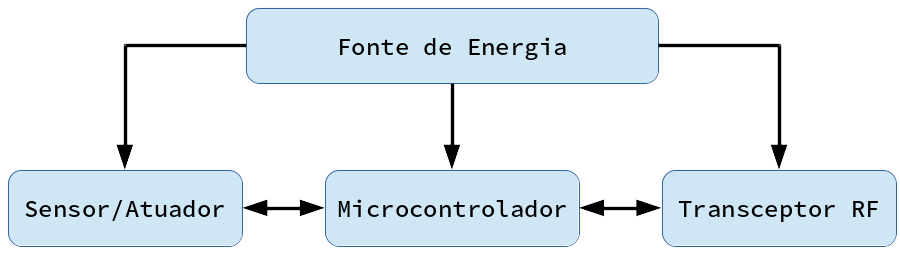
\includegraphics[scale=0.5]{../images/node.png}
	\hspace{\linewidth}
	Fonte: elaborada pelo autor
	\label{figura:node}
\end{figure}

\subsection{Microcontrolador}
Microcontroladores são geralmente definidos como computadores completos em um único \textit{chip}, pois
consistem de um núcleo de processamento com memórias de dados e de programa, pinos de E/S configuráveis e
outras funcionalidades, dependendo do modelo utilizado, como temporizadores, portas de comunicação serial,
conversor analógico-digital, etc \cite{williams2014,kuorilehto2007}.

Além disso, algumas características como flexibilidade em conectar dispositivos externos, conjunto de
instruções favoráveis à processamento de tempo-crítico e baixo consumo elétrico fazem com que os MCUs sejam
amplamente utilizados em diversas aplicações, como sistemas embarcados e, evidentemente, redes de sensores sem
fio \cite{karl_willig2005}.

Atualmente, existem inúmeros modelos de MCU de fabricantes diferentes no mercado, e um dos mais populares são
os modelos \texttt{AVR} da empresa \textit{Atmel Corporation}. O principal motivo pela difusão desses modelos,
além do baixo preço, é que eles oferecem \textit{softwares} abertos e gratuitos para realizar a implementação
do código embarcado. Um deles é o compilador \texttt{avr-gcc}, que é uma montagem do \textit{GNU Compiler Collection}
específica para os AVR e utiliza a biblioteca \texttt{AVR-Libc}, que fornece um subconjunto da biblioteca C
padrão. Além disso, há também o programa \texttt{avrdude}, que é o responsável em transferir o código binário
gerado para o microcontrolador.

Conforme mostra a figura \ref{figura:avr}, os microcontroladores AVR estão disponíveis em diversos tamanhos e
pacotes, sendo que as funcionalidades embutidas, quantidade de memória disponível e outros atributos dependem
do modelo utilizado.

\begin{figure}[h]
	\caption{Microcontroladores AVR}
	\centering
	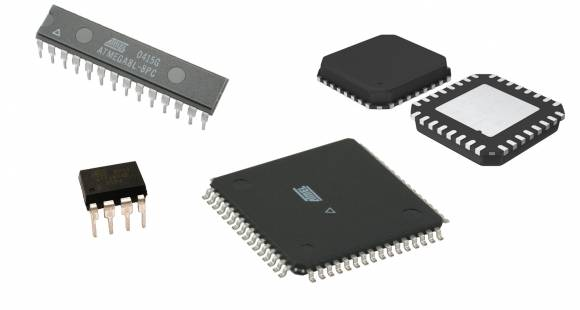
\includegraphics[scale=0.5]{../images/avr.jpg}
	\hspace{\linewidth}
	Fonte: http://home.roboticlab.eu
	\label{figura:avr}
\end{figure}

Os modelos AVR são os mesmos utilizados pelo Arduino, que nada mais é que uma camada de abstração ao MCU e que
oferece algumas facilidades como conectores mais convenientes, bibliotecas implementadas, entre outras.
Contudo, o objetivo principal do Arduino é permitir que novatos e pessoas fora da área possam realizar
prototipações de computação de baixo nível. Embora seja uma ótima plataforma, seu custo chega a ser quatro vez
mais que um AVR separado \cite{trevennor2012}.

\subsection{Sensor/Atuador}
Ver Capítulo \ref{cap:3}.

\subsection{Transceptor}
O uso da comunicação por radiofrequcência (RF) tem se tornado cada vez mais abrangente, indo desde as
aplicações tradicionais, como transmissão de sinais de rádio e televisão, para as mais diversas utilidades,
como monitoramento de pacientes em um hospital, \textit{mouses} e teclados sem fio, identificação por
radiofrequência (RFID) e, naturalmente, redes de sensores sem fio \cite{misra2001}.

Embora transceptores baseados em ondas ópticas possuam uma eficiência energética melhor, sua necessidade por
uma condição de linha de visão devido ao seu comportamento direcional faz com que a comunicação baseada em RF
seja a mais relevante para a construção de uma RSSF, pois, além de ser omnidirecional, provê uma distância de
alcance e uma taxa de tranferência de dados relativamente grandes \cite{kuorilehto2007,karl_willig2005}.

Conforme mencionado no Capítulo \ref{cap:1}, os módulos transceptores RF que implementam protocolos de
comunicação avançados como o ZigBee e o Wi-Fi deixam a desejar em relação ao preço e consumo energético,
sendo necessário optar por módulos mais simples.

Uma possibilidade é utilizar o transceptor \texttt{CC2500} da empresa \textit{Texas Instruments}, que
implementa o padrão IEEE 802.15.4 e possui uma taxa máxima de transmissão aérea de 500 Kbps, consumindo
\SI{17}{\milli \ampere} durante recepção, \SI{21.2}{\milli \ampere} durante transmissão e \SI{1.5}{\milli
\ampere} em modo de espera. Devido ao baixo consumo elétrico e ótimo custo-benefício, esse dispositivo é
amplamente utilizado. \cite{ccdatasheet}

Outro transceptor de rádio frequência bastante difundido é o \texttt{nRF24L01+} da empresa \textit{Nordic
Semiconductor}. Embora possui a desvantagem de não seguir o padrão aberto da IEEE, esse dispositivo apresenta
diversas vantagens em relação aos demais módulos dessa categoria. Uma das principais vantagens é sua taxa
máxima de transmissão aérea de 2 Mpbs (quatro vezes mais que o \texttt{CC2500}) e que, ao mesmo tempo, consome
menos energia elétrica que os demais, sendo \SI{13.5}{\milli \ampere} durante recepção, \SI{11.3}{\milli
\ampere} durante transmissão e \SI{26}{\micro \ampere} em modo de espera. \cite{nrfdatasheet}

Além disso, o \texttt{nRF24L01+}, ilustrado na figura \ref{figura:nrf}, oferece serviços como reconhecimento e
retransmissão de pacotes automáticos, diminuindo o número de comunicação com a unidade microtronladora tal
como o processamento utilizado pela mesma. Dessa forma, além de reduzir ainda mais o consumo elétrico
necessário, possibilita uma implementação eficiente utilizando microcontroladores simples e baratos.

\begin{figure}[h]
	\caption{Transceptor NRF24L01+}
	\centering
	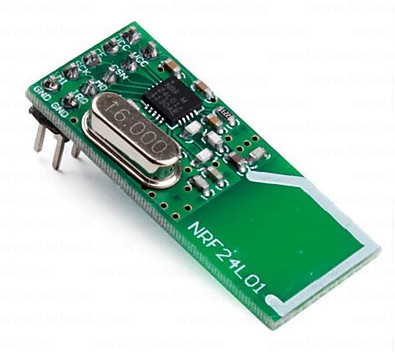
\includegraphics[scale=0.25]{../images/nrf.jpg}
	\hspace{\linewidth}
	Fonte: http://www.techmake.com
	\label{figura:nrf}
\end{figure}

\subsection{Fonte de Energia}
